\paragraph{QuizziPedia::Front-End::Views::LoginView}
\begin{figure} [ht]
	\centering
	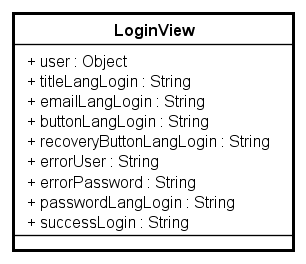
\includegraphics[scale=0.80]{UML/Classi/Front-End/QuizziPedia_Front-end_Views_LoginView.png}
	\caption{QuizziPedia::Front-End::Views::LoginView}
\end{figure} \FloatBarrier
\begin{itemize}
	\item \textbf{Descrizione}: view contenente le form necessarie per effettuare il login. Contiene inoltre un link alla pagina di registrazione e uno alla pagina per il recupero della password;
	\item \textbf{Utilizzo}: premette all'utente di autenticarsi inserendo username e password;
	\item \textbf{Relazioni con altre classi}:
	\begin{itemize}
		\item \textit{IN} \texttt{LoginModelView}: classe di tipo modelview la cui istanzazione è contenuta all'interno della variabile di ambiente \$scope di \texttt{Angular.js}. All'interno di essa sono presenti le variabili e i metodi necessari per il \textit{Two-Way Data-Binding\ped{G}} tra la view \texttt{LoginView} e il controller \texttt{LoginController};
		\item \textit{IN} \texttt{LangModel}: rappresenta il modello delle informazioni per la giusta traduzione dell'applicazione.
	\end{itemize}
	\item \textbf{Attributi}:
	\begin{itemize}
		\item \texttt{+ user: Object} \\ Campo dati contenente due attributi: \texttt{username: String} e \texttt{password: String};
		\item \texttt{+ titleLangLogin: String} \\ Attributo che viene utilizzato per visualizzare la giusta traduzione del titolo della pagina, in italiano o in inglese;
		\item \texttt{+ emailLangLogin: String} \\ Attributo che viene utilizzato per visualizzare la giusta traduzione della \textit{label\ped{G}} per l'inserimento dell'email, in italiano o in inglese;
		\item \texttt{+ passwordLangLogin: String} \\ Attributo che viene utilizzato per visualizzare la giusta traduzione della \textit{label\ped{G}} per l'inserimento della password, in italiano o in inglese;  
		\item \texttt{+ buttonLangLogin: String} \\ Attributo che viene utilizzato per visualizzare la giusta traduzione della \textit{label\ped{G}} per il bottone di autenticazione, in italiano o in inglese;
		\item \texttt{+ recoveryBottonLangLogin: String} \\ Attributo che viene utilizzato per visualizzare la giusta traduzione della \textit{label\ped{G}} per il bottone di link al recupero della password, in italiano o in inglese;
		\item \texttt{+ successLogin: String} \\ Attributo che visualizza un messaggio di avvenuta registrazione;
		\item \texttt{+ errorUser: String} \\ Attributo che visualizza un eventuale messaggio di errore nell'inserimento dell'email, in italiano o in inglese;
		\item \texttt{+ errorPassword: String} \\ Attributo che visualizza un eventuale messaggio di errore nell'inserimento della password, in italiano o in inglese.
	\end{itemize}
\end{itemize}